%!TEX root = ../../../main.tex
%%---------------------------------------------------------------------------
\section{Human Machine Interface}
\label{sec:rc_hmi}
%%---------------------------------------------------------------------------
-Develop an interface for the robot cell capable of:\\
-Monitor the robot components current state and position.\\
-Monitor and parameter adjustments of the camera system.\\
-Manually control the robot, conveyor and gripper position and state\\
-Inform the MES server of the robot availability state\\
-Manual or automatic mode.\\
-Overall equipment effectiveness parameters\\	

	\begin{figure}[H]
		\centering
	    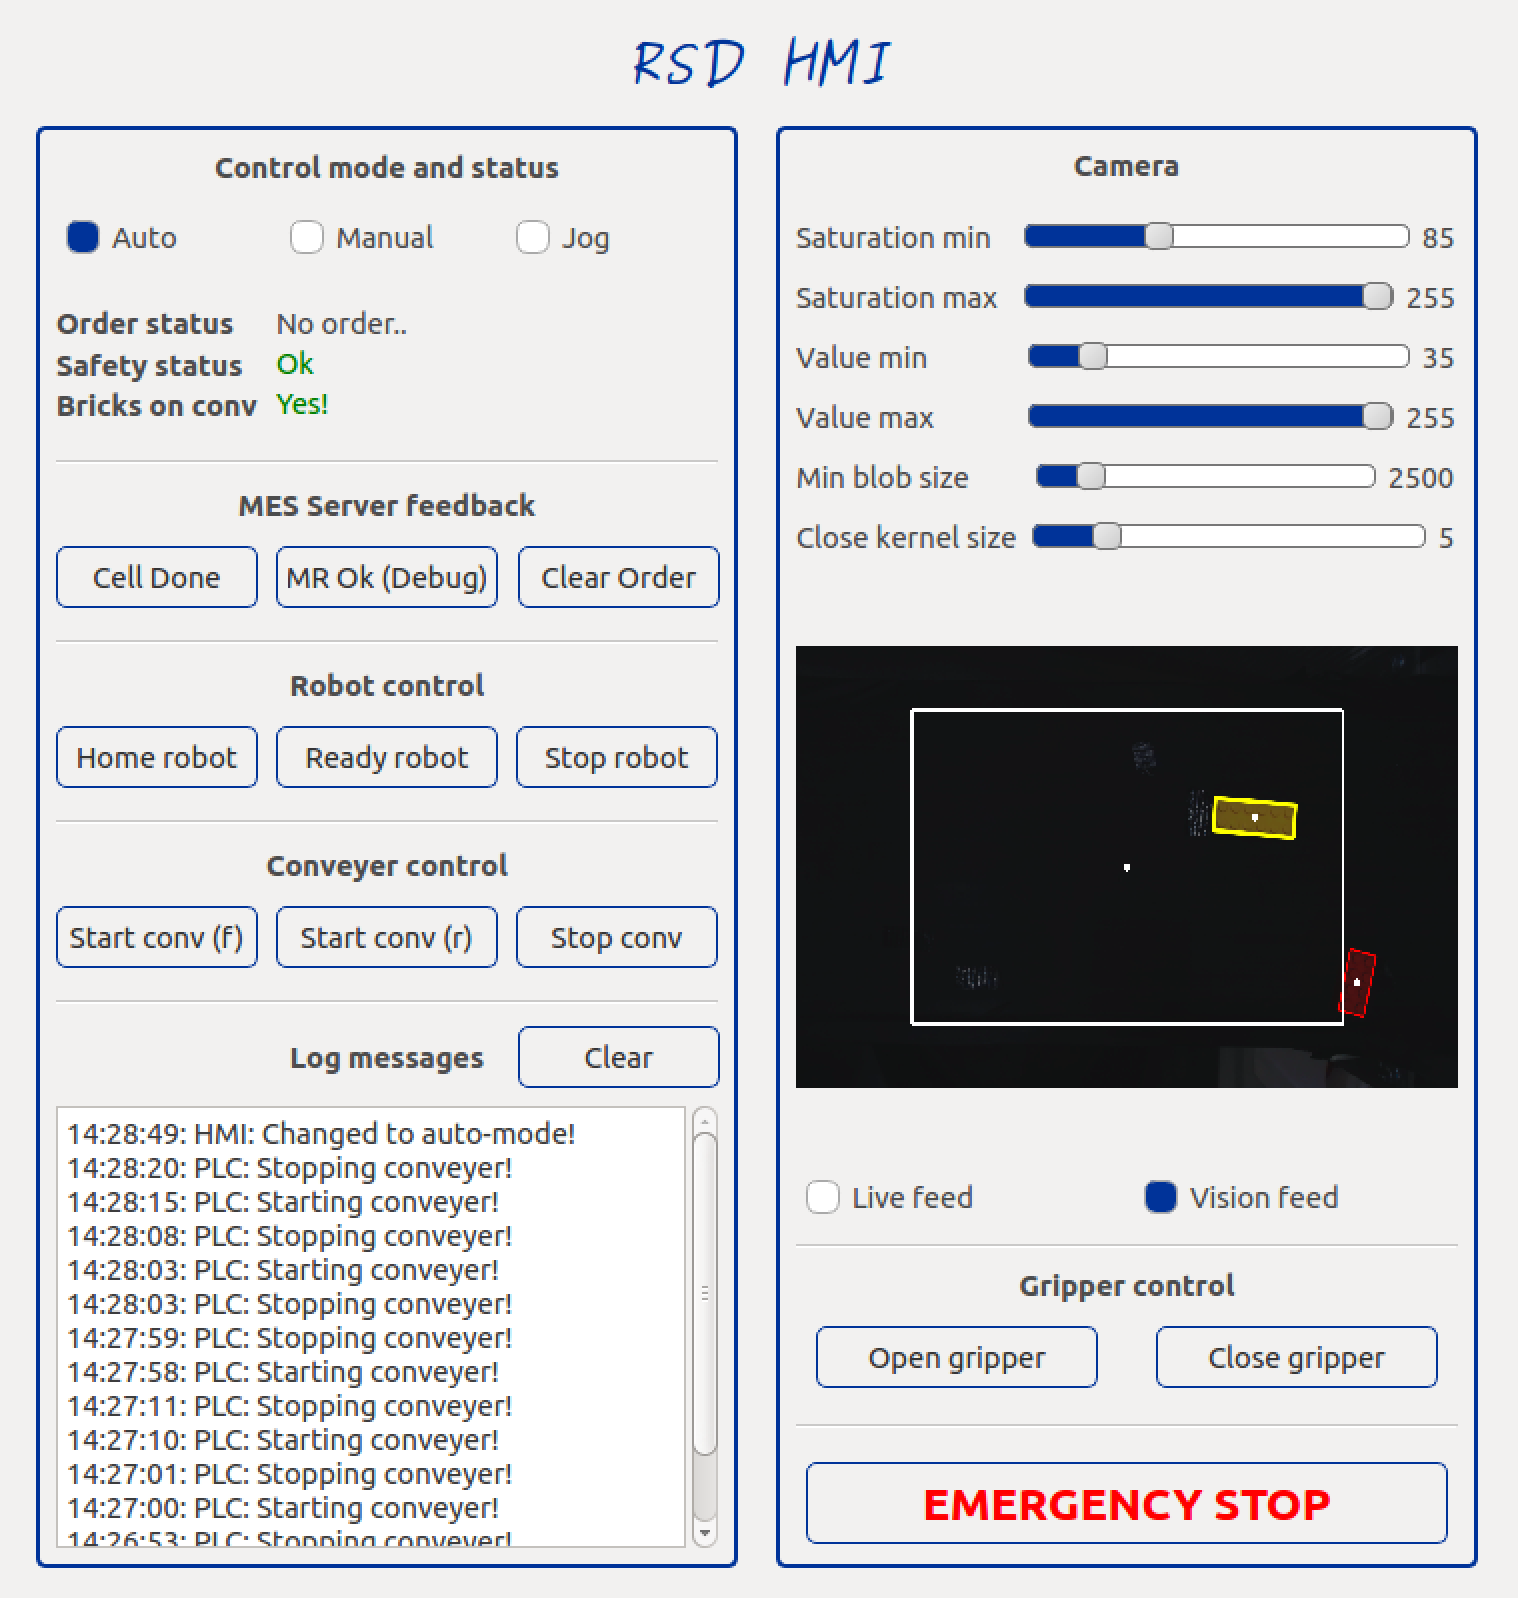
\includegraphics[width=0.95\textwidth]{rc_hmi}
	    \caption{HMI}
		\label{fig:rc_hmi}
	\end{figure}
	
	\begin{figure}[H]
		\centering
	    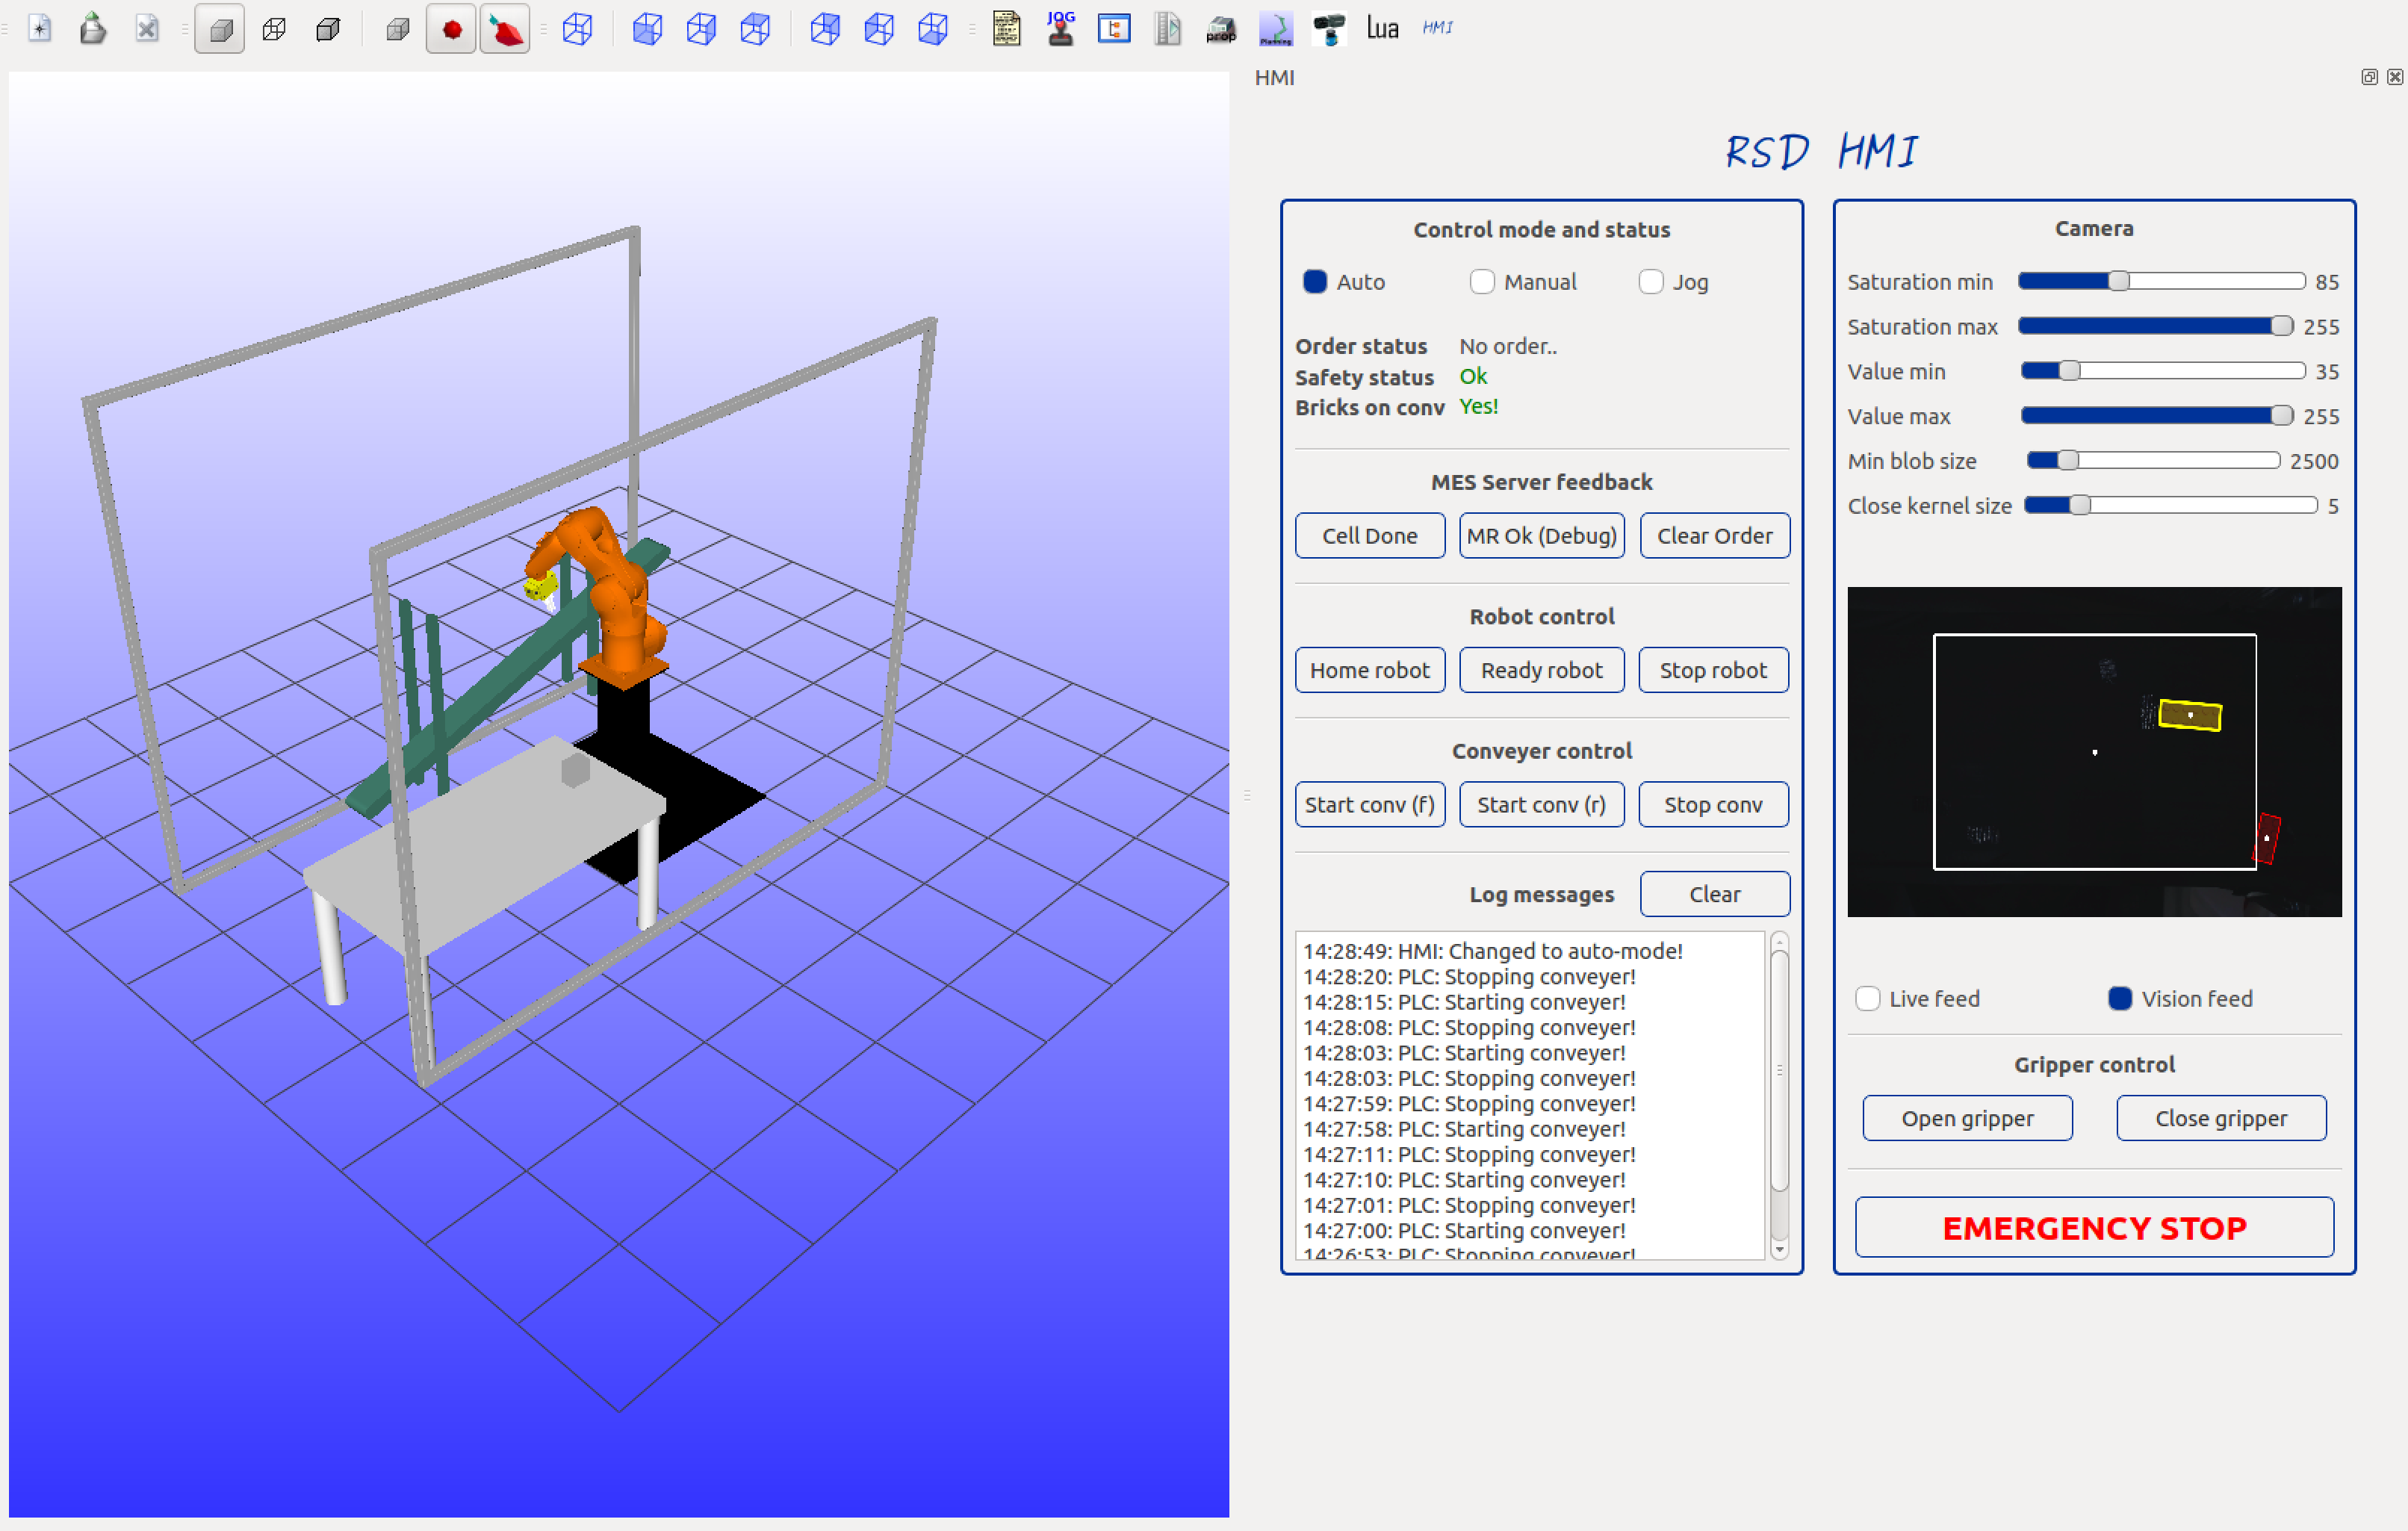
\includegraphics[width=0.95\textwidth]{rc_hmi_full}
	    \caption{Full HMI with simulated work-cell shown}
		\label{fig:rc_hmi_full}
	\end{figure}